%!TeX root = main.tex
%!encoding = UTF-8 Unicode

\section{LISN Measurement for System-Level Cross Reference}

This section presents the LISN measurements as a cross-reference to the intrinsic emission measurements.
As an example, a \SI{1200}{V} SiC MOSFET in a D2PAK package is used as the DUT, and the standard gate-resistance variation test is performed.
Since the oscilloscope ground is fixed to the aluminum base plate, no current measurement is carried out in this configuration.
The measurement results are shown in \fref{fig:MR_LISN_Voltage_TD} and \fref{fig:MR_LISN_LISN_TD} for the time domain and in \fref{fig:MR_LISN_FD} for the frequency domain.

\begin{figure}[ht]
	\centering
	\tikzsetnextfilename{MR_LISN_Voltage_TD}
	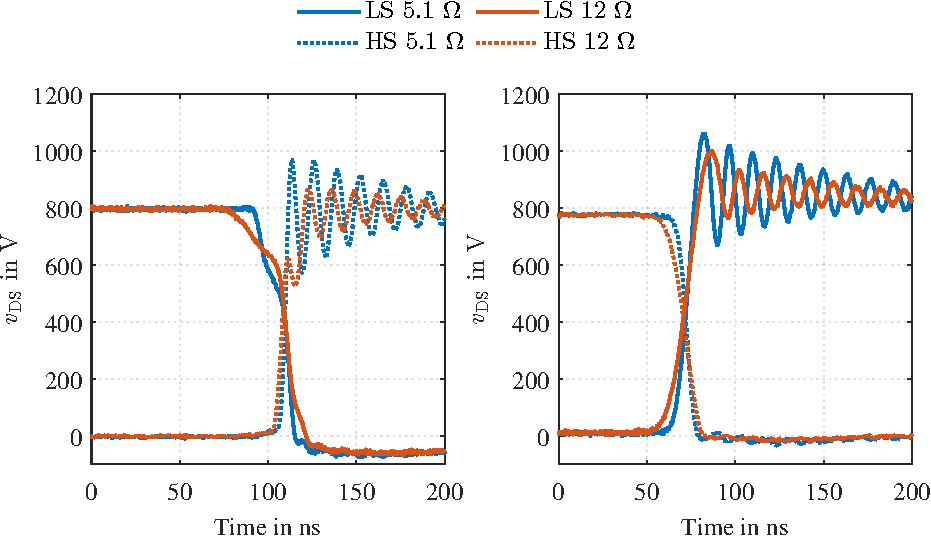
\includegraphics[scale=1]{figures/6_Environment/MR_LISN/MR_LISN_Voltage_TD.pdf}
	\caption{Time-domain measurement of low-side and high-side voltages for two gate resistances at \SI{800}{V} and \SI{60}{A} for PMTX03.}\label{fig:MR_LISN_Voltage_TD}
\end{figure}

\begin{figure}[ht]
	\centering
	\tikzsetnextfilename{MR_LISN_LISN_TD}
	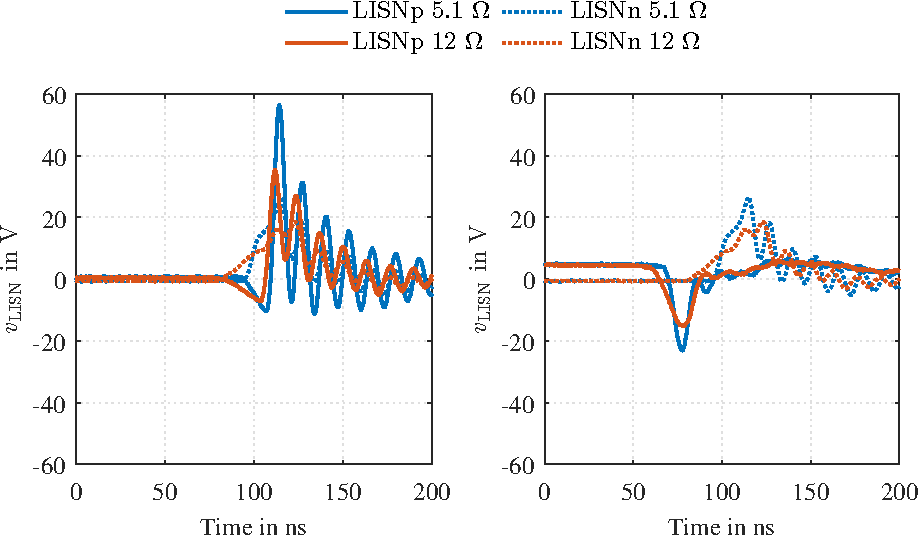
\includegraphics[scale=1]{figures/6_Environment/MR_LISN/MR_LISN_LISN_TD.pdf}
	\caption{Time-domain measurement of LISN voltages for two gate resistances at \SI{800}{V} and \SI{60}{A} for PMTX03.}\label{fig:MR_LISN_LISN_TD}
\end{figure}

The time-domain plots confirm the expected influence of increased gate resistance: the switching speed decreases and the voltage transitions become slower.
This is the classical behavior observed in gate-resistance variation studies.
In contrast, the frequency-domain plots provide more relevant information for EMC analysis, because they reveal how system-level parasitics and return paths shape the emission behavior.
These LISN measurements represent the state of the art for semiconductor-oriented EMC analysis, and their limitations are discussed in the following.

The upper graph of \fref{fig:MR_LISN_FD} shows the intrinsic emissions measured with the high-pass output of the DAVP.
The lower two graphs show the conventional LISN voltages, first directly and then in the translated common-mode and differential-mode components.
The corresponding voltages can be calculated as
\begin{equation}
    \mi{v}{CM} = \frac{1}{2}\cdot(\mi{v}{LISNp} + \mi{v}{LISNn})
\end{equation}

\begin{equation}
    \mi{v}{DM} = \frac{1}{2}\cdot(\mi{v}{LISNp} - \mi{v}{LISNn})
\end{equation}

When the LISN voltages are examined, the onset of the noise floor becomes evident slightly above the resonance frequency at \SI{75}{MHz}.
This noise floor is the same as the one introduced in Sec.~\ref{sec:methods} and is only marginally lower than that of a direct drain-source voltage measurement, because the switching node couples capacitively to the cooler and then to the LISN terminals.
However, this creates a first-order transfer function, while the actual signal falls with second-order or even higher-order behavior.
This is clearly visible in the high-pass measurement of the drain-source voltages, which span a much wider range from \SI{40}{dB\mu V} to \SI{140}{dB\mu V}, compared to only about \SI{30}{dB} for the LISN voltages.
Consequently, the maximum measurable frequency in the system-level measurement with the LISN is approximately \SI{150}{MHz}, while the DAVP measures up to \SI{400}{MHz}.

\begin{figure}[ht]
	\centering
	\tikzsetnextfilename{MR_LISN_FD}
	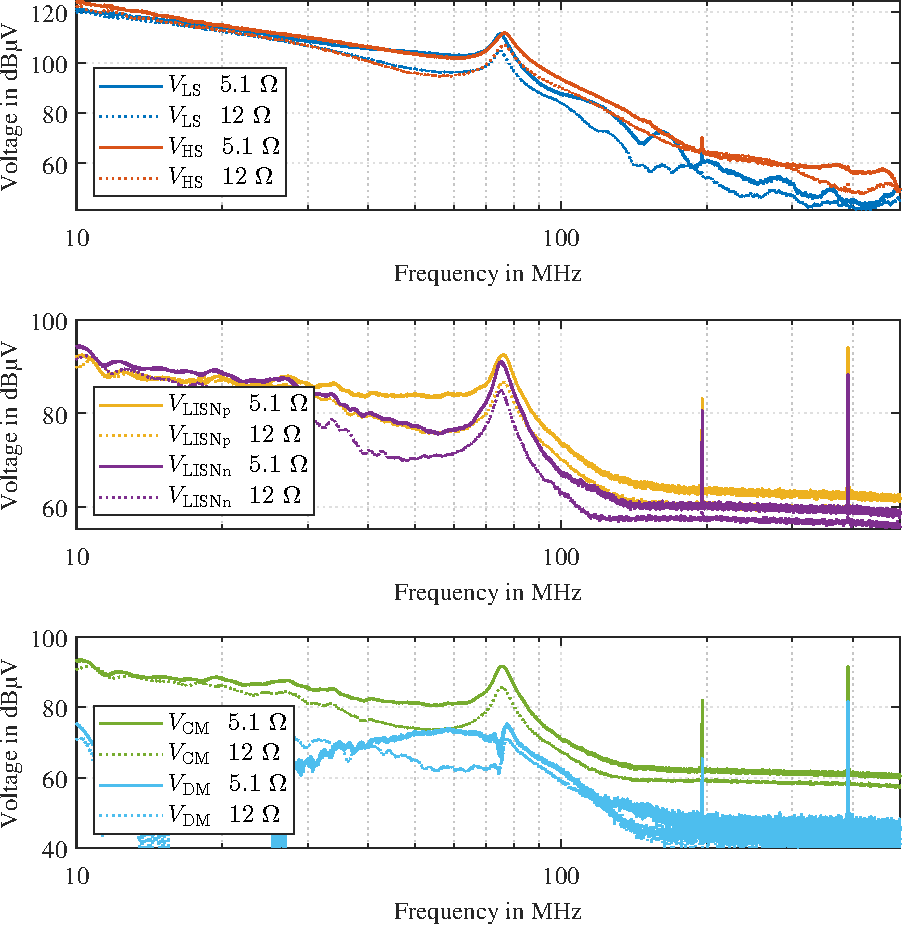
\includegraphics[scale=1]{figures/6_Environment/MR_LISN/MR_LISN_FD.pdf}
	\caption{Frequency-domain measurement of drain-source and LISN voltages for two gate resistances at \SI{800}{V} and \SI{60}{A} for PMTX03.}\label{fig:MR_LISN_FD}
\end{figure}

Nevertheless, some additional insight can be gained from the data.
When the high-side and low-side main resonances are compared, a small mismatch in resonance frequency becomes visible.
This is caused by passive turn-off, where the oscillation couples into the gate and the corresponding capacitances create a slight mismatch.
This effect does not occur during active turn-off, because the gate driver holds the gate capacitance constant.
This behavior is discussed in detail in \cite{paper}.
A similar mismatch can also be observed in the LISN voltages.
While the peak of \mi{v}{LISNp} occurs at \SI{76}{MHz}, the peak of \mi{v}{LISNn} occurs at \SI{74}{MHz}, which corresponds exactly to the resonances of \mi{v}{DS,HS} and \mi{v}{DS,LS}, respectively.
This can be explained by the positioning of the high-side and low-side MOSFETs relative to the positive and negative LISN terminals.
From \fref{fig:pic_b2b_setup}, it is evident that the high-side switch \mi{Q}{HS} is placed closer to LISNp, while \mi{Q}{LS} is placed closer to LISNn.
The respective noise of each switch therefore follows the lowest-impedance or shortest return path.
Furthermore, the general slope of the raw emission \mi{v}{DS} is also visible in the system-level measurements \mi{v}{LISN}, confirming the validity of the complete measurement approach.

In future work, the transfer function between these two measurement types should be investigated.
This would enable system-level information to be extracted from raw emission measurements and extend the usable range of this approach.





